\section{C3PO in Perspective}
As part of this thesis a software prototype is developed that aims to tackle the issues, problems and gaps presented in the previous chapters. The aim is to create a tool that is able to automatically generate a colletion profile of bigger collections (consisting of hundreds of thousands or even millions of objects). 

This profile includes a descriptive statistical representation of the content in the collection, meaning that it contains very specific data such as count of objects, overall size of objects, etc. Furthermore, it provides histogramms of different aspects of the content, such as the file formats, mimetypes, and many other ordinal characteristics that are of interest to the user of the application.

On top of that a service layer enables the user to query the tool in order to gain a deeper insight into the content. This may include the filtering of the content based on different characteristics and splitting it into buckets, which will allow to compare homogeneous parts (based on one or more characteristika) in an otherwise heterogenous content. 

Visualizations and multi dimensional representations of these filterings enable to user to understand the profile and thus provide her with the fundamental knowledge and a more stable ground to take more efficient decisions.
The prototype implementation of the tools is called 'Clever, Crafty Content Profiling of Objects' or c3po for short and is presented in detail in the following subsections.
% idea
% overview
% part of scape, watch source, etc..

\section{Architecture}
In this chapter an overview over the architecture of c3po and its more important aspects are presented.

\subsection{High Level Overview}
C3po is separated into different modules and provides a relatively simple workflow that follows the three steps of content profiling as presented in (TODO cite). In the first part it gathers raw meta data and parses it in order to normalize it into a simple internal data model. In the next step the data is cleaned up, partially aggregated and stored into an external to the tool database.
This offers the baseline for the more deeper analysis provided by some of the modules.


\begin{figure}[htb]
\begin{center}
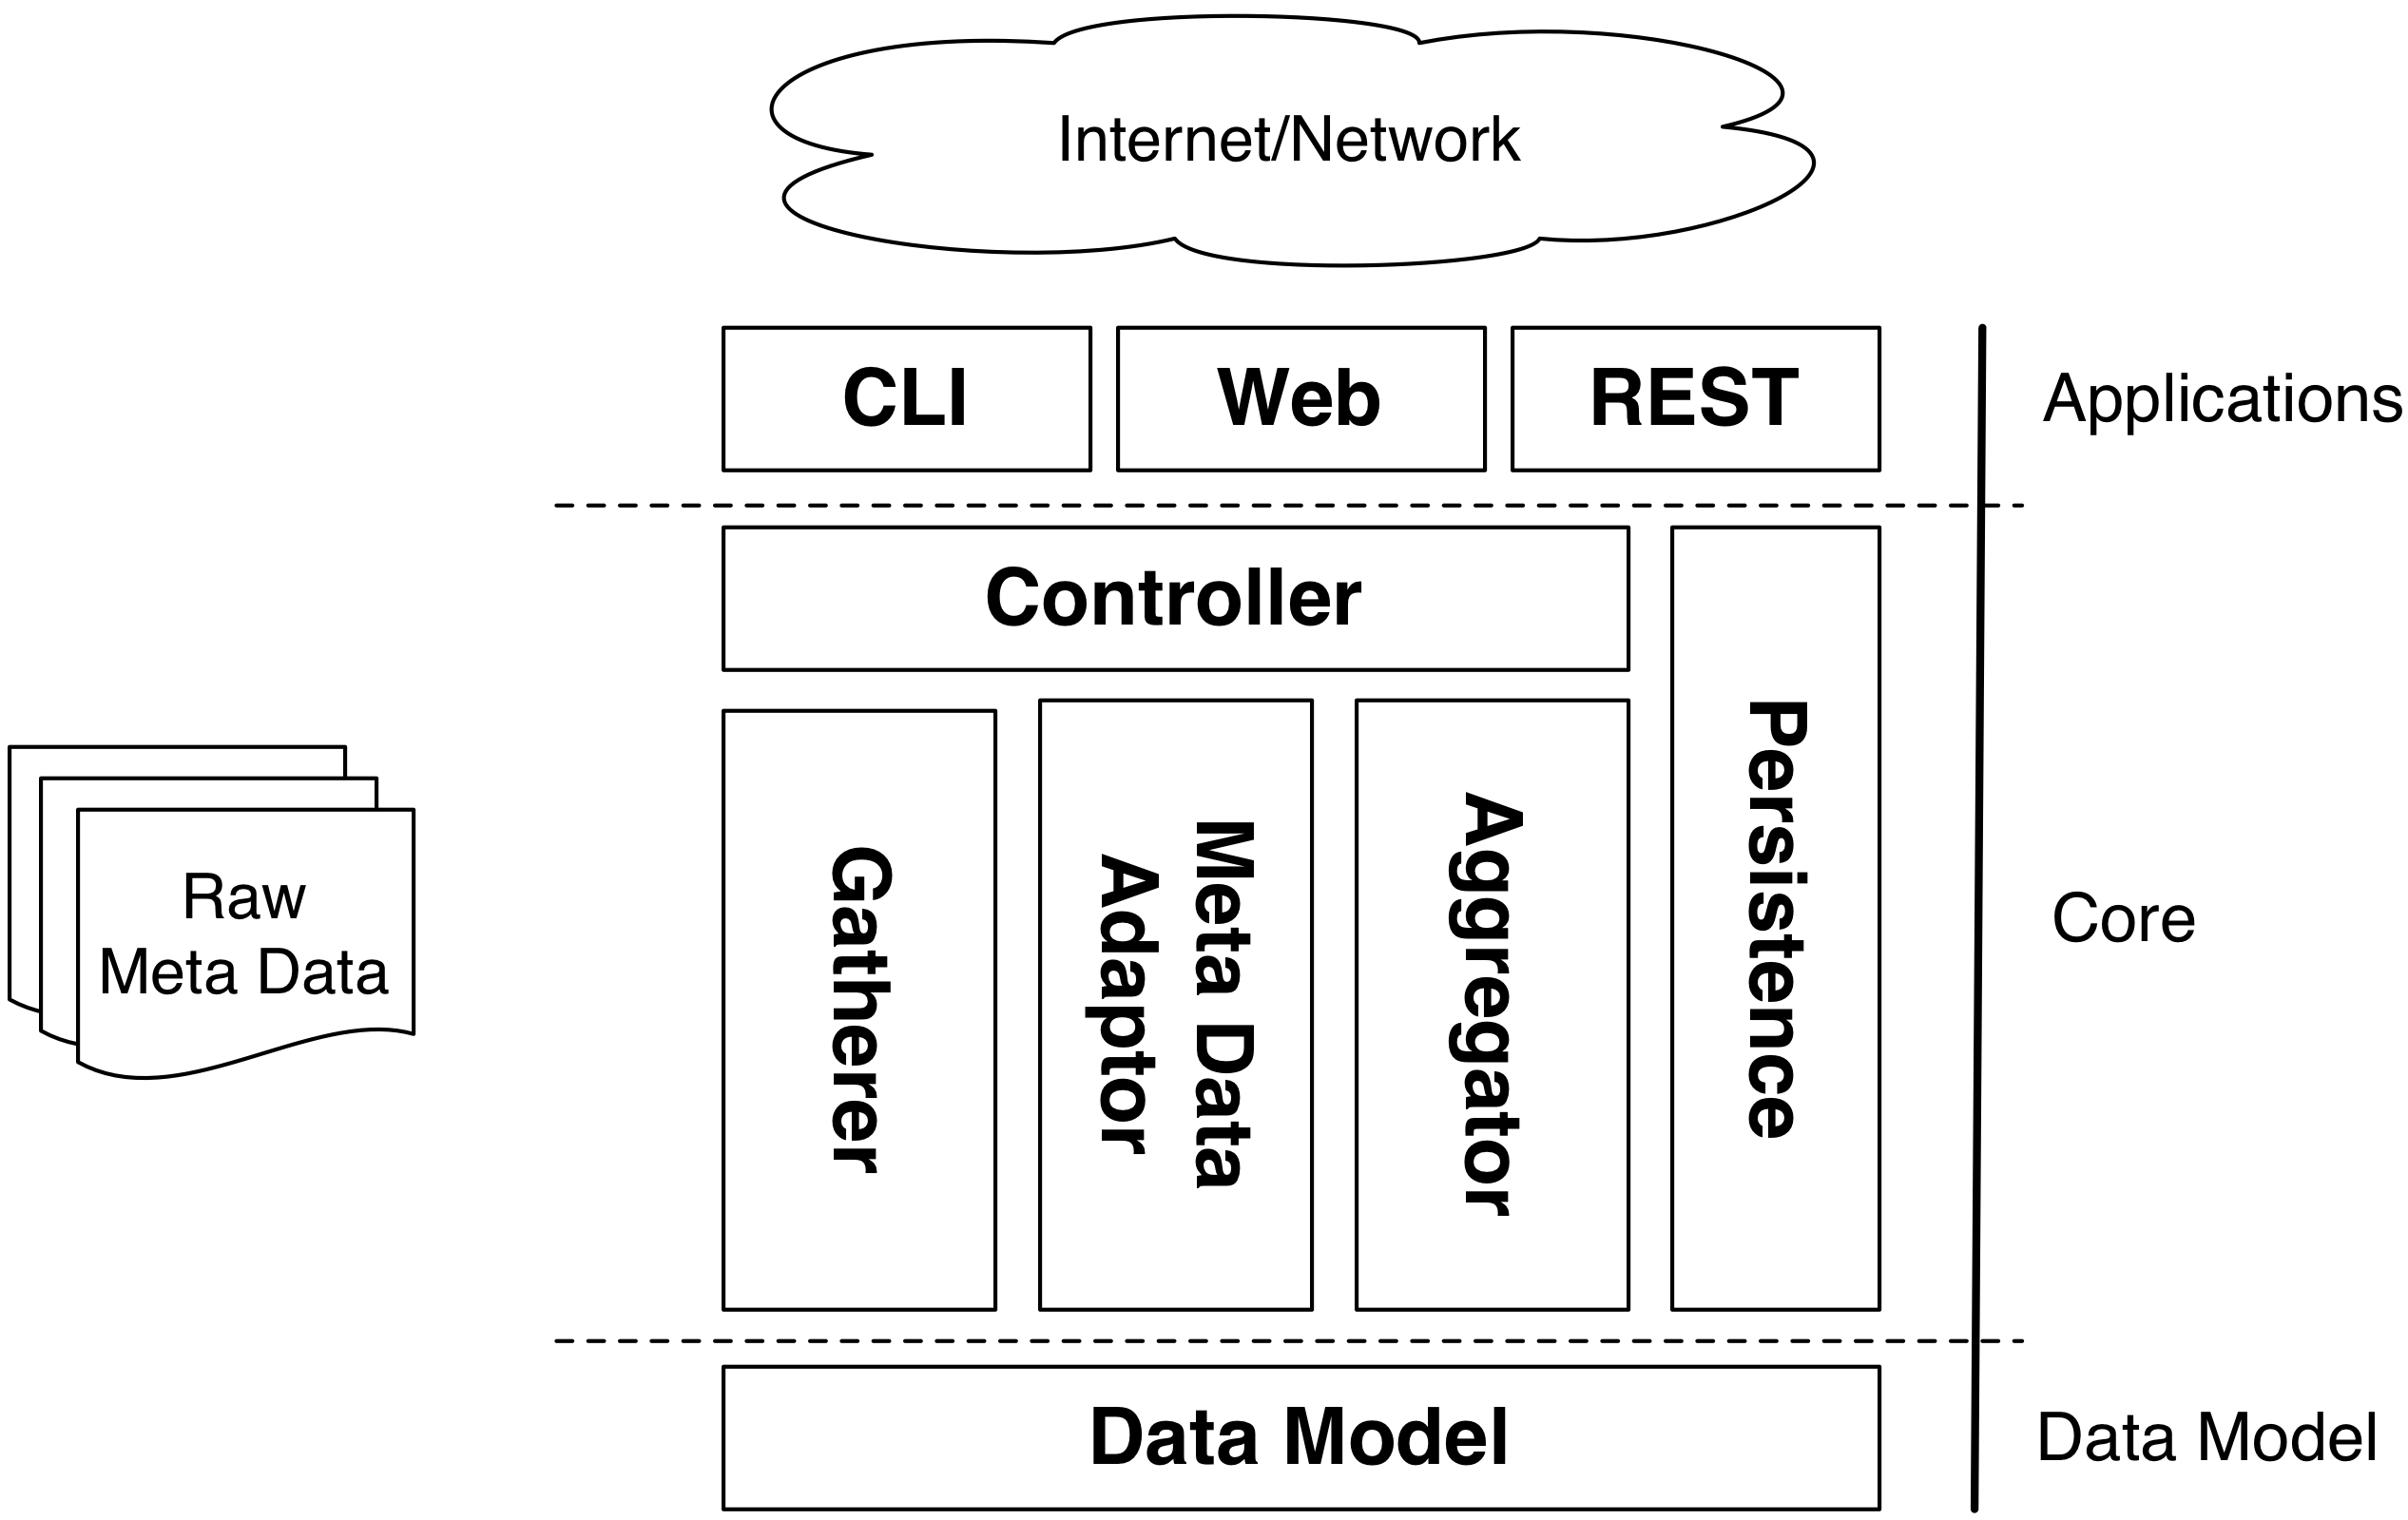
\includegraphics[width=5in]{figures/architecture/c3po_highlevel_architecture.png}
\caption{High-level architecture of c3po.}
\label{fig:architecture_highlevel}
\end{center}
\end{figure}

Figure \ref{fig:architecture_highlevel} presents the high level architecture and its modules. At the bottom there is the domain model module which sits as the foundation of the architecture. It represents a simple model able to capture the important aspects of the content meta data in a more generic way but still provides the ability to do flexible queries over the data. It consists mainly of elements - the digital objects and values representing the measurements of specific meta data characteristics. The complete model is provided in (TODO section).

Above that is the main part or the core module, which encapsulates the framework that allows the gathering, normalizing and aggregation of the data. It not only offers interfaces that allow the extension of the framework but also it provides the glue-ware to create and run the work flow.
On top, there is a simple controller, that uses the components below to carry out the work flow. Currently it is implemented in a single threaded, sequential manner, but a potential parallelization is considered in the design as a potential performance optimization.

Below that, there are three important components: the Gatherer, the Meta Data Adaptor and the Aggregator component.
As described in section (TODO cite) the raw meta data of the content can be stored in many different places or sources. For example, it can be provided locally in form of files stored on the local file system, or remotely. The remote source can have many different variations. E.g. there can be a remote ssh server that stores the raw meta data again in file form, or a remote web archive server that stores the meta data in special container files called arc or warc file, but there can be also a remote repository, which not only stores the original content but all the meta data for each object in a different way (internal db, to its local fs, etc.). The latter represents the most likely use case in a real world digital preservation scenario, however all others are possible as well, not to mention that they are easier to use for experimentation purposes.

As c3po is not interested in the way of how and where the meta data is stored, the gatherer component offers an interface, which provides an abstraction to all these differences and exposes a unified interface allowing the Controller to obtain streams to the next N files that have to be processed. Currently c3po provides implementations only for local file systems, however extending the tool to be able to fetch data from a different source is just a matter of implementing a single interface, which is able to count the files to be processed and to open streams to the next N files. 
%Eventually, say that there is no restriction currently of how the implementation shall look like, e.g. direct stream over the network or  temporary storage to the local system.

Since different sources can use different characterization tools and different characterization tool outputs, the Meta Data Adaptor component is responsible for instantiating and assigning a specific implementation of an adaptor that can handle the gathered meta data records. Currently c3po is based on the FITS output format as described in (TODO cite). Extending to other formats should be pretty straight forward and a matter of a new adaptor implementation.

% TODO implement and describe aggregator.

The last part of the core module is the persistence layer. C3po's persistence is based on the Java Persistence API\footnote{http://docs.oracle.com/javaee/6/tutorial/doc/bnbpz.html} (JPA 1.0) with Hibernate\footnote{http://www.hibernate.org/} as the persistence provider. The higher level abstraction is done via a couple of generic data access object (DAO) interfaces, which have to be implemented by the client application, or client module.
This might seem a bit odd at first look, as it is partly strange to leave the core part without a concrete implementation that handles such an important and fundamental part as data storage. However, there is a very specific reason, why this design was chosen.

The c3po tool is meant to be deployable in application servers, so that queries by other tools and users can be done over the network. For this, a special container managed transactional model is needed. On the other hand, content profiling is a data intensive process, which can gain from the fact that the tool can execute near the data. That is why, also a local transactional model is needed, in which the tool is run locally near the data without any application server. All this allows the separation of the data gathering and the data analysis parts of the work flow. The fact that the data base is external to the tool also means that it can be setup near the data or on a specific storage sever that has enough resources at its hand to handle the load.

There is a simple command line application that offers an implementation of c3po persistence layer apis/daos and also there is the web module, which has a container managed implementation. The web module represents the last part of the tool, where a simple web application that exposes some of the functionality of the tool over a REST (TODO cite) interface. REST was chosen for two main reasons. For one, it is easy to understand and pretty straightforward to implement. This allows easy integration with other tools, such as monitoring services (TODO cite) and a variety of client applications. The second reason is that other technologies, such as JSF and EJBs would have meant that only a few application servers will be compliant and able to support the application. As already mentioned, easy deployment is part of the requirements and thus the implementation shall avoid relying on frameworks that are restricting the choice of the server.
%REST cite: http://www.ics.uci.edu/~fielding/pubs/dissertation/rest_arch_style.htm

\subsection{Data Model}

\subsection{Interfaces and Extension Points}

\subsection{Build Process and Deployment}
The separation of the high level architecture into modules is not only done in a logical fashion. By using a widely spread and used build management tool called Maven\footnote{http://maven.apache.org} the code is separated into different packages, that can be found here: (TODO link). Maven is responsible for fetching and managing all the dependencies and their correct versions for c3po.
All this makes the distribution and maintainability of the application much easier as well as it provides an easy build process.

Currently the deployment requires a standard distribution of a Java Application Server and the copying of one war packed into the deployment directory.

\section{Representative Set Algorithm 1}

\section{Representative Set Algorithm 2}

\section{Comparison \& Evaluation}

\section{Future Points of Interest}
% scalability
% continious profiling
% input to simulator
% ...
